\documentclass{article} % For LaTeX2e
\usepackage{nips12submit_e,times}
%\documentstyle[nips12submit_09,times,art10]{article} % For LaTeX 2.09
\usepackage{graphicx}
\usepackage{amsmath,amssymb}
\usepackage{subfigure}

\usepackage{xcolor}
\newcommand{\X}{\mathcal{X}}
\newcommand{\reals}{\mathbb{R}}
\newcommand{\GaP}{\text{GaP}}
\newcommand{\Ga}{\text{Ga}}
\newcommand{\idf}[1]{\mathbf 1 \left ( #1 \right )}
\newcommand{\E}{\mathbb{E}}
\newcommand{\K}{\mathcal{K}}
%\newcommand{\Y}{\mathcal{Y}}
\newcommand{\bigspace}{\mathcal{X} \times \Theta \times \reals^+}
\newcommand{\Un}{\text{Un}}
\newcommand{\scrF}{\mathcal{F}}
\newcommand{\norm}[1]{\left | \left | #1 \right | \right |}
\newcommand{\N}{\text{N}}


\title{Slice sampling normalized kernel-weighted completely random measure
mixture models}


\author{
Nicholas J.~Foti \\
Department of Computer Science\\
Dartmouth College\\
Hanover, NH 03755 \\
\texttt{nfoti@cs.dartmouth.edu} \\
\And
Sinead A. Williamson \\
Department of Machine Learning \\
Carnegie Mellon University \\
Pittsburgh, PA 15213 \\
\texttt{sinead@cs.cmu.edu} \\
}

% The \author macro works with any number of authors. There are two commands
% used to separate the names and addresses of multiple authors: \And and \AND.
%
% Using \And between authors leaves it to \LaTeX{} to determine where to break
% the lines. Using \AND forces a linebreak at that point. So, if \LaTeX{}
% puts 3 of 4 authors names on the first line, and the last on the second
% line, try using \AND instead of \And before the third author name.

\newcommand{\fix}{\marginpar{FIX}}
\newcommand{\new}{\marginpar{NEW}}

\nipsfinalcopy % Uncomment for camera-ready version

\begin{document}


\maketitle

\begin{abstract}
  A number of dependent nonparametric processes have been
  proposed to model non-stationary data with unknown latent dimensionality.
  However, the inference algorithms are often slow and unwieldy, and are in
  general highly specific to a given model formulation. In this paper, we
  describe a large class of dependent nonparametric processes, including several existing
  models, and present a slice sampler that allows efficient inference across
  this class of models.
\end{abstract}

% Body
\section{Introduction} 

Nonparametric mixture models allow us to bypass the
issue of model selection, by modeling data using a random number of mixture components
that can grow if we observe more data. However, such models work on the
assumption that data can be considered exchangeable. This assumption often does
not hold in practice as distributions commonly vary with some covariate. For
example, the proportions of different species may vary across geographic
regions, and the distribution over topics discussed on Twitter is likely to 
evolve over time.

Recently, there has been increasing interest in \emph{dependent} nonparametric
processes \cite{MacEachern:1999}, that extend existing nonparametric
distributions to non-stationary data. While a nonparametric process is a
distribution over a single measure, a dependent nonparametric process is a
distribution over a \emph{collection} of measures, which may be associated with
values in a covariate space. The key property of a dependent nonparametric
process is that the measure at each covariate value is marginally distributed
according to a known nonparametric process.

A number of dependent nonparametric processes have been developed in the
literature (\cite{Dunson:2010} $\S6$). For example, the single-p DDP \cite{MacEachern:1999} defines a
collection of Dirichlet processes with common atom sizes but variable atom
locations. The order-based DDP \cite{Griffin:Steel:2006} constructs a collection of
Dirichlet processes using a common set of beta random variables, but permuting
the order in which they are used in a stick-breaking construction. The Spatial
Normalized Gamma Process (SNGP) \cite{Rao:Teh:2009} defines a gamma process on
an augmented space, such that at each covariate location a subset of the atoms
are available. This creates a dependent gamma process, that can be normalized
to obtain a dependent Dirichlet process. The kernel beta process (KBP)
\cite{Ren:Wang:Dunson:Carin:2011}
defines a beta process on an augmented space, and at each covariate location
modulates the atom sizes using a collection of kernels, to create a collection 
of dependent beta processes.

Unfortunately, while such models have a number of appealing properties,
inference can be challenging. While there are many similarities between
existing dependent nonparametric processes, most of the inference schemes that
have been proposed are highly specific, and cannot be generally applied without
significant modification. 

The contributions of this paper are twofold.  First, in Section~\ref{sec:dep}
we describe a general class of dependent nonparametric processes, based on
defining completely random measures on an extended space.  This class of models
includes the SNGP and the KBP as special cases. Second, we develop a
slice sampler that is applicable for all the dependent probability measures in
this framework. We compare our slice sampler to existing inference algorithms,
and show that we are able to achieve superior performance over existing
algorithms. Further, the generality of our algorithm mean we are able to easily
modify the assumptions of existing models to better fit the data, without the
need to significantly modify our sampler.

%\begin{itemize}
%\item Why dependent nonparametric models are useful.
%\item Briefly mention existing DDPs and CRMs
%\item Inference difficulties
%\item Summary of contributions:
%  \begin{itemize}
%  \item Define a class of dependent normalized random measures that includes the SNGP as a special case.
%  \item Develop a slice sampling algorithm that can be generally applied and has good performance.
%\end{itemize}
%\end{itemize}


%\section{Background}
\subsection{Completely random measures and normalized random measures}
A completely random measure (CRM, CITE:KINGMAN) is a distribution over
discrete\footnote{with, possibly, a deterministic continuous component} measures
$B$ on some measureable space $\Omega$ such that, for any disjoint subsets
$A_k\in\Omega$, the masses $B(A_k)$ are independent. Commonly used examples of
CRMs include the gamma process, the generalized gamma process, the beta process,
and the stable process. A CRM is uniquely categorized by a L\'{e}vy measure
$\nu$ on $\Omega\times\reals_+$, which controls the location and size of the
jumps. We can interpret a CRM as a Poisson process on $\Omega\times\reals_+$
with mean measure $\nu$.

A distribution over probability measures can be obtained by normalizing the
random measure $B$. Such distributions are often referred to as normalized
random measures (NRM, CITE:KINGMAN). The most commonly used example of an NRM is
the Dirichlet process, which can be obtained as a normalized gamma process.
Other CRMs yield NRMs with different properties -- for example a normalized
gamma process can have heavier tails than a Dirichlet process (IS THIS TRUE?
DETAILS ABOUT SOME OTHER NRMs).

Most research attention has focused on the Dirichlet process, due in part to its
conjugacy to the multinomial distribution which allows us to develop a number of
samplers. More recently, SOMETHING ABOUT THE JAMES PSEUDO-CONJUGACY RESULTS FOR
NRMS. This has led to the development of efficient auxiliary variable inference
algorithms for arbitrary NRMs. (CITE: GRIFFIN, OTHERS)

%\subsection{Dependent nonparametric processes}
%Most nonparametric priors, such as the Dirichlet process, gamma process, or beta process, are used to model a single dataset, that is assumed to be exchangeable. Dependent nonparametric processes [CITE: MACEACHERN NDP PAPER) extend such priors to give distributions over \emph{collections} of datasets, which may be associated with values in a covariate space. The key property of a dependent nonparametric process is that the marginal distribution at each covariate value is distributed according to a known nonparametric process.

%A number of dependent nonparametric processes have been developed in the literature. For example, the single-p DDP [CITE:MACEACHERN] defines a collection of Dirichlet processes with common atom sizes but variable atom locations. The order-based DDP [CITE:GRIFFIN] constructs a collection of Dirichlet processes using a common set of beta random variables, but permuting the order in which they are used in a stick-breaking construction. The Spatial Normalized Gamma Process (SN$\Gamma$P, CITE:RAO/TEH) defines a gamma process on an augmented space, such that at each covariate location a subset of the atoms are available. This creates a dependent gamma process, that can be normalized to obtain a dependent Dirichlet process. The kernel beta process (KBP, CITE) defines a beta process on an augmented space, and at each covariate location modulates the atom sizes using a collection of kernels, to create a collection  of dependent beta processes.

%Unfortunately, while such models have a number of appealing properties, inference can be challenging. [COMMENT ON INFERENCE] In Section~\ref{sec:dep} we describe a general class dependent nonparametric processes, based on defining completely random measures on an extended space.  This class of models includes the KBP and the SN$\Gamma$P as special cases. We develop a slice sampler that is applicable for all normalized random measures in this framework, and demonstrate that the sampler achieves at least as good solutions as obtained by existing methods and runs much faster.
%DO WE WANT TO GO INTO SPECIFIC DETAILS HERE ABOUT THE SNGP AND KBP?


\section{Constructing dependent nonparametric models using kernels}\label{sec:dep}

In this section, we describe a general class of dependent completely random
measures, that includes the kernel beta process as a special case. We then
describe the class of dependent normalized random measures obtained by
normalizing these dependent completely random measures, and show that the SNGP
lies in this framework.

\subsection{Kernel CRMs}
A completely random measure (CRM) \cite{Kingman:1967,LijoiPrunster:2009} is a distribution over
discrete\footnote{with, possibly, a deterministic continuous component} measures
$B$ on some measurable space $\Omega$ such that, for any disjoint subsets
$A_k\subset\Omega$, the masses $B(A_k)$ are independent. Commonly used examples of
CRMs include the gamma process, the generalized gamma process, the beta process,
and the stable process. A CRM is uniquely categorized by a L\'{e}vy measure
$\nu(d\omega,d\pi)$ on $\Omega\times\reals_+$, which controls the location and size of the
jumps. We can interpret a CRM as a Poisson process on $\Omega\times\reals_+$
with mean measure $\nu(d\omega,d\pi)$.

Let $\Omega = (\X \times \Theta)$, and let $\Pi = \{(\mu_k,\theta_k,\pi_k)\}_{k=1}^\infty$ be a Poisson process on the
space $\bigspace$ with associated product $\sigma$-algebra.  The space has
three components: $\X$, a bounded space of covariates; $\Theta$, a space of
parameter values; and $\reals^+$, the space of atom masses.  Let the 
mean measure of $\Pi$ be described by the positive L\'evy
measure $\nu(d\mu,d\theta,d\pi)$.  While the construction herein applies for
any such L\'evy measure, we focus on the class of L\'evy measures that
factorize as $\nu(d\mu,d\theta,d\pi) = R_0(d\mu)H_0(d\theta)\nu_0(d\pi)$.  This
corresponds to the class of homogeneous CRMs, where the size of an atom is
independent of its location in $\Theta \times \X$, and covers most CRMs
encountered in the literature.  We assume that $\X$ is a discrete space with
$P$ unique values, $\mu^*_p$, in order to simplify the exposition, and without
loss of generality we assume that $R_0(\X)=1$.  Additionally,
let $K(\cdot,\cdot) : \X \times \X \rightarrow [0,1]$ be a bounded kernel
function.  Though any such kernel may be used, for
concreteness we only consider a box kernel and square exponential kernel
defined as
\begin{itemize}
  \item{\textbf{Box kernel:}}
    $K(x,\mu) = \idf{\norm{x-\mu} < W}$, where we call $W$ the width.
  \item{\textbf{Square exponential kernel:}}
    $K(x,\mu) = \exp \left ( -\psi \norm{x-\mu}^2 \right )$, for 
    $\norm{\cdot}$ a dissimilarity measure, and $\psi > 0$ a fixed
    constant.
\end{itemize}


Using the setup above we define a kernel-weighted CRM (KCRM) at a fixed
covariate $x \in \X$ and for $A$ measurable as
\begin{equation}
\textstyle  B_x(A) = \sum_{m=1}^\infty K(x,\mu_m)\pi_m \delta_{\theta_m}(A)
  \label{eqn:kcrm}
\end{equation}
which is seen to be a CRM on $\Theta$ by the mapping theorem for Poisson
processes \cite{Kingman:1993}.  For a fixed set of observations $(x_1,\ldots,x_G)^T$
we define $\mathcal{B}(A) = (B_{x_1}(A),\ldots,B_{x_G}(A))^T$ as the vector of
measures of the KCRM at the observed covariates.
CRMs are characterized by their
characteristic function (CF) \cite{FristedtGray:1997} which for the 
CRM $\mathcal{B}$ can be written as
\begin{equation}
  \E[\exp(-v^T\mathcal{B}(A))] = \exp \left ( -\int_{\X \times A \times \reals^+}
  (1-\exp(-v^T\K_\mu\pi)\nu(d\mu,d\theta,d\pi))\right )
  \label{eqn:kcrmcf}
\end{equation}
where $v \in \reals^G$ and $\K_\mu = (K(x_1,\mu),\ldots,K(x_G,\mu))^T$.
Equation \ref{eqn:kcrmcf} is easily derived from the general form of the CF of
a Poisson process \cite{Kingman:1993} and by noting that the one-dimensional CFs are 
exactly those of the individual $B_{x_i}(A)$.  
%Equation \ref{eqn:kcrmcf} is necessary for the derivation of the slice sampler.  
See \cite{Ren:Wang:Dunson:Carin:2011} for a discussion of the dependence structure
between $B_x$ and $B_{x'}$ for $x,x' \in \X$.

Taking $\nu_0$ to be the L\'evy measure of a beta process \cite{Hjort:1990} results
in the KBP.  Alternatively, taking $\nu_0$ as the L\'evy measure of a
gamma process, $\nu_{\text{GaP}}$ \cite{Ferguson:1973}, and $K(\cdot,\cdot)$ as the
box kernel we recover the unnormalized form of the SNGP.

\subsection{Kernel NRMs}
\label{sec:dNRM} 

A distribution over probability measures can be obtained by starting from a
CRM, and normalizing the resulting random measure.
Such distributions are often referred to as normalized random measures (NRM)
\cite{Regazzini:Lijoi:Prunster:2003}. The most commonly used example of an NRM is the Dirichlet
process, which can be obtained as a normalized gamma process
\cite{Ferguson:1973}.  Other CRMs yield NRMs with different properties -- for
example a normalized generalized gamma process can have heavier tails than a Dirichlet
process \cite{LijoiMenaPrunster:2007}.

We can define a class of dependent NRMs in a similar manner, starting from the
KCRM defined above. Since each marginal measure $B_x$ of $\mathcal{B}$ is a
CRM, we can normalize it by its total mass, $B_x(\Theta)$, to produce a NRM
\begin{equation} 
  P_x(A) = B_x(A) / B_x(\Theta) = \sum_{m=1}^\infty
  \frac{K(x,\mu_m)\pi_m}{\sum_{l=1}^\infty K(x,\mu_l)\pi_l}\delta_{\theta_m}(A)
  \label{eqn:nkcrm} 
\end{equation} 
This formulation of a kernel NRM (KNRM) is
similar to that in \cite{Griffin:2007} for Ornstein-Uhlenbeck NRMs (OUNRM).
While the OUNRM framework allows for arbitrary CRMs, in theory,
extending it to arbitrary kernel functions is non-trivial.
A fundamental difference between OUNRMs and normalized KCRMs is that the 
marginals of an 
OUNRM follow a specified process, whereas the marginals of a KCRM may be
different than the underlying CRM.

A common use in statistics and machine learning for NRMs is as prior
distributions for mixture models with an unbounded number of components
\cite{FavaroTeh:2012}.  Analogously, covariate-dependent NRMs can be used as priors for
mixture models where the probability of being associated with a mixture
component varies with the covariate \cite{Rao:Teh:2009,Griffin:2007}.  For concreteness, we
limit ourselves to a kernel gamma process (KGaP) which we denote as
$\mathcal{B} \sim \text{KGaP}(K, R_0, H_0, \nu_{\text{GaP}})$, although the
slice sampler can be adapted to any normalized KCRM.

Specifically, we observe data $\{(x_j,y_j)\}_{j=1}^N$ where $x_j \in \X$
denotes the covariate of observation $j$ and $y_j \in \reals^d$ denotes
the quantities we wish to model.  Let $x^*_g$ denote the $g$th unique covariate
value among all the $x_j$ which induces a partition on the observations
so that observation $j$ belongs to group $g$ if $x_j = x^*_g$.  We
denote the $i$th observation corresponding to $x^*_g$ as $y_{g,i}$.

Each observation is associated with a mixture component which we denote as
$s_{g,i}$ which is drawn according to a normalized KGaP on a parameter space
$\Theta$, such that $(\theta,\phi) \in \Theta$, where $\theta$ is a mean and $\phi$
a precision.
Conditional on $s_{g,i}$, each observation is then drawn from some density
$q(\cdot|\theta,\phi)$ which we assume to be $\N(\theta,\phi^{-1})$.  The full model
can then be specified as 
\begin{equation}
  \begin{aligned} 
    P_g(A) | \mathcal{B} &\sim B_g(A)/B_g(\Theta) \\
    s_{g,i} | P_g &\sim \sum_{m=1}^\infty \frac{ K(x^*_g,\mu_m)\pi_m }
    { \sum_{l=1}^\infty K(x^*_g,\mu_l)\pi_l } \delta_{m} \\
    (\theta^*_m,\phi^*_m) &\sim H_0(d\theta,d\phi) \\
    y_{g,i} | s_{g,i}, \{(\theta^*,\phi^*)\} &\sim 
    q(y_{g,i}|\theta^*_{s_{g,i}},\phi^*_{s_{g,i}}) 
  \end{aligned}
  \label{eqn:mixmod}
\end{equation}

If $K(\cdot,\cdot)$ is a box kernel, Eq.~\ref{eqn:mixmod} describes a
SNGP mixture model \cite{Rao:Teh:2009}.

\section{A slice sampler for dependent NRMs}

The slice sampler of \cite{GriffinWalker:2011} allows us to perform inference in arbitrary
NRMs. We extend this slice sampler to perform inference in the class of
dependent NRMs described in Sec.~\ref{sec:dNRM}.  The slice sampler can be used with any
underlying CRM, but for simplicity we concentrate on an underlying gamma
process, as described in Eq.~\ref{eqn:mixmod}.
In the supplement we also derive a Rao-Blackwellized estimator of
the predictive density for unobserved data using the output from the slice
sampler.  We use this estimator to compute predictive densities in the
experiments.

Analogously to \cite{GriffinWalker:2011} we introduce a set of auxiliary
slice variables -- one for each data point. Each data point can only belong to
clusters corresponding to atoms larger than its slice variable. The set of
slice variables thus defines a minimum atom size that need be represented,
ensuring a finite number of instantiated atoms.

We extend this idea to the KNRM framework. Note that, in this case, an atom
will exhibit different sizes at different covariate locations. We refer to
these sizes as the \emph{kernelized atom sizes}, $K(x_g^*,\mu)\pi$, obtained by
applying a kernel $K$, evaluated at location $x^*_g$, to the raw atom $\pi$.
Following~\cite{GriffinWalker:2011}, we introduce a local slice variable $u_{g,i}$. This allows
us to write the joint distribution over the data points $y_{g,i}$, their
cluster allocations $s_{g,i}$ and their slice variables $u_{g,i}$ as 
\begin{align}
  f({\mathbf y}, {\mathbf u}, {\mathbf s} | \pi, \mu, \theta, \phi) &=
  \prod_{g=1}^G V_g^{n_g-1} e^{(-V_g B_{Tg})} \prod_{i=1}^{n_g} \idf{ u_{g,i}
  < K(x^*_g,\mu_{s_{g,i}})\pi_{s_{g,i}} } q(y_{g,i} | \theta_{s_{g,i}},
  \phi_{s_{g,i}})
  \label{eqn:slicealmost}
\end{align}
where $B_{Tg} = B_{x^*_g}(\Theta) = \sum_{m=1}^\infty K(x_g^*,\mu_m)\pi_m$ and $V_g \sim \Ga(n_g,B_{Tg})$ 
is an auxiliary variable\footnote{We parametrize the gamma
distribution so that $X \sim \Ga(a,b)$ has mean $a/b$ and variance
$a/b^2$}.  
See the supplement and \cite{GriffinWalker:2011,JamesLijoiPrunster:2009} for a 
complete derivation.

In order to evaluate Eq.~\ref{eqn:slicealmost}, we need to evaluate $B_{Tg}$,
the total mass of the unnormalized CRM at each covariate value. This involves
summing over an infinite number of atoms -- which we do not wish to represent.
Define $0 < L = \min{\{u_{s_{g,i}}\}}$. This gives the smallest possible
(kernelized) atom size to which data can be attached. Therefore, if we
instantiate all atoms with raw size greater than $L$, we will include all atoms
associated with occupied clusters. For any value of $L$, there will be a finite
number $M$ of atoms above this threshold. From these $M$ raw atoms, we can
obtain the kernelized atoms above the slice corresponding to a given data
point.

We must obtain the remaining mass by marginalizing over all kernelized atoms
that are below the slice (see the supplement).  We can
split this mass into, \textbf{a}.) the mass due to atoms that are not instantiated (i.e. whose kernelized value
is below the slice at all covariate locations)
and, \textbf{b}.) the mass due to currently instantiated atoms (i.e. atoms
whose kernelized value is above the slice at at least one covariate location)
\footnote{If $\X$ were not 
bounded there would be a third term consisting of raw atoms $> L$ that when
kernelized fall below the slice everywhere.  These can be ignored by a
judicious choice of the space $\X$ and the allowable kernel widths.}. As we show in the supplement, the first term, \textbf{a}, 
corresponds to atoms
$(\pi,\mu)$ where $\pi < L$, the mass of which can be written as
\begin{align}
  \sum_{\mu^* \in \X} \left ( R_0(\mu^*) \int_0^L (1-\exp{(-V^T
  \K_{\mu^*}\pi)})\nu_0(d\pi) \right )
  \label{eqn:Ltail}
\end{align}
where $V = (V_1, \ldots, V_G)^T$. This can be evaluated numerically for many 
CRMs including gamma and generalized
gamma processes \cite{GriffinWalker:2011}.
The second term, \textbf{b}, consists of realized atoms $\{(\pi_k,\mu_k)\}$ such that 
$K(x^*_g,\mu_k)\pi_k < L$ at covariate $x^*_g$.  We use a Monte Carlo estimate
for \textbf{b} that we describe in the supplement.
For box kernels term \textbf{b} vanishes, and we have found that even for the
square exponential kernel ignoring this term yields good results.

\subsection{Sampling equations}

Having specified the joint distribution in terms of a finite measure with a
random truncation point $L$ we can now describe a sampler that samples in turn
from the conditional distributions for the auxiliary variables $V_g$, the gamma
process parameter $\alpha = H_0(\Theta)$, the instantiated raw atom 
sizes $\pi_m$ and
corresponding locations in covariate space $\mu_m$ and in parameter space
$(\theta_m, \phi_m)$, and the slice variables $u_{g,i}$.  We define some
simplifying notation: $\K_\mu = (K(x_1^*,\mu),\ldots, K(x_G^*,\mu))^T$; $B_+ = (B_{+1},\ldots,B_{+G})^T$, 
$B_* = (B_{*1},\ldots,B_{*G})^T$, where  $B_{+g} =
\sum_{m=1}^M K(x^*_g,\mu_m)\pi_m$, $B_{*g} = \sum_{m=M+1}^\infty
K(x^*_g,\mu_m)\pi_m$ so that $B_{Tg} = B_{+g} + B_{*g}$; and $n_{g,m} =
|\{s_{g,i} : s_{g,i} = m, i \in 1,\ldots,n_g\}|$.
\begin{itemize} 
  \item \textbf{Auxiliary variables} $V_g$: The full conditional distribution 
    for $V_g$ is given by
    \begin{equation} p(V_g \, | \, n_g, V_{-g}, B_+, B_*) \propto
      V_g^{n_g-1}\exp(-V^TB_+)\E[\exp(-V^TB_*)], \; V_g > 0 
      \label{eqn:postvg}
    \end{equation} 
    which we sample using Metropolis-Hastings moves,
    as in \cite{GriffinKolSteel:2010}.

  \item \textbf{Gamma process parameter} $\alpha$: The conditional distribution 
  for $\alpha$ is given by
  \begin{equation}
    \begin{aligned}
      p(\alpha \, | \, K, V, \mu,\pi) \propto p(\alpha)\alpha^K 
       %\exp \left ( -\alpha \int_L^\infty \left [ 1 + 
       % \int_\X (1-e^{(-V^T \K_\mu\pi)}) R_0(d\mu) \right ] \nu_0(d\pi) \right )
       e^{ -\alpha \left [ \int_L^\infty \nu_0(d\pi) + 
        \int_0^L \int_\X (1-\exp{(-V^T \K_\mu\pi)}) R_0(d\mu) \nu_0(d\pi) \right ] }
    \end{aligned}
  \end{equation}
  If $p(\alpha) = \Ga(a_0,b_0)$ then the posterior is also a gamma
  distribution with parameters
  \begin{align}
    \label{eqn:postalphaa}
    a &= a_0 + K \\
    b &= b_0 + \int_L^\infty \nu_0(d\pi) + 
    \int_\X \int_0^L (1-\exp(-V^T \K_\mu\pi))\nu_0(d\pi)  R_0(d\mu)
    \label{eqn:postalphab}
  \end{align}
  where the first integral in Eq.~\ref{eqn:postalphab} can be 
  evaluated for many processes of interest and the second integral can be
  evaluated as in Eq.~\ref{eqn:Ltail}.
  \item \textbf{Raw atom sizes} $\pi_m$: The posterior for atoms associated with 
    occupied clusters is given by
    \begin{align}
      p(\pi_m \, | \, n_{g,m}, \mu_m, V, B_+) &\propto\pi_m^{\sum_{g=1}^G n_{g,m}} \exp \left (
      -\pi_m \sum_{g=1}^G V_gK(x^*_g,\mu_m) \right )
      \nu_0(\pi_m)
      \label{eqn:pipost}
    \end{align}
    For an underlying gamma or generalized gamma process, the posterior of
    $\pi_m$ will be given by a gamma distribution due to conjugacy
    \cite{GriffinWalker:2011}.
    There will also be a number of atoms with raw size $\pi_m>L$ that do not have
    associated data. The number of such atoms is Poisson distributed with mean 
    $\alpha \int_A \exp ( -V^T \K_\mu \pi)\nu_0(d\pi)R_0(d\pi)$, where 
    $A = \{(\mu,\pi) : K(x^*_g,\mu)\pi > L, \text{ for some } g\}$ and which can be 
    computed using the approach described for Eq.~\ref{eqn:Ltail}.
  \item \textbf{Raw atom covariate locations} $\mu_m$: Since we assume a finite set 
    of covariate locations, we can sample $\mu_m$ according to the discrete 
    distribution
    %the conditional distribution
    \begin{align}
      p(\mu_m \, | \, n_{g,m}, V, B_+) \propto \prod_{g=1}^G K(x^*_g,\mu_k)^{n_{g,m}} \exp \left ( -\pi_m
      \sum_{g=1}^K V_g K(x^*_g,\mu_m) \right ) R_0(\mu_m)
      \label{eqn:postmu}
    \end{align}
  %can be evaluated (up to a constant) for each location, allowing us to sample 
  %the value of $\mu_m$ according to a discrete distribution.
  \item \textbf{Slice variables} $u_{g,i}$: Sampled as 
    $u_{g,i}  | \{\pi\}, \{\mu\}, s_{g,i} \sim \Un[0, K(x^*_g, \mu_{s_{g,i}})
    \pi_{s_{g,i}}]$. %We then set $L = \min{u_{g,i}}$.
  \item \textbf{Cluster allocations} $s_{g,i}$: The prior on $s_{g,i}$ cancels with
    the prior on $u_{g,i}$, yielding
  \begin{equation}
    p(s_{g,i} = m \, | \, y_{g,i}, u_{g,i}, \theta_m, \pi_m, \mu_m) \propto
        q(y_{g,i}|\theta_m,\phi_m) \idf{u_{g,i} < K(x^*_g,\mu_m)\pi_m}
        \label{eqn:post_s}
      \end{equation}
      where only a finite number of $m$ need be evaluated.

  \item \textbf{Parameter locations}: Can be sampled as in a standard mixture 
    model \cite{GriffinWalker:2011}.
\end{itemize}

\section{Experiments}

We evaluate the performance of the proposed slice sampler in the setting of
covariate dependent density estimation.  We assume 
the statistical
model in Eq.~\ref{eqn:mixmod} and consider a univariate Gaussian
distribution as the data generating distribution.  We use both synthetic and
real data sets in our experiments and compare the slice sampler to a Gibbs
sampler for a finite approximation to the model (see the supplement
for details of the model and sampler) and to the original SNGP sampler.
We assess the mixing
characteristics of the sampler using the integrated autocorrelation time $\tau$ of the
number of clusters used by the sampler at each iteration after a burn-in
period, and by the predictive quality of the collective samples on held-out
data.  The integrated autocorrelation time
of samples drawn from an MCMC algorithm
controls the Monte Carlo error inherent in a sample drawn from the MCMC
algorithm.  It can be shown that in a set of $T$ samples from the MCMC
algorithm, there are in effect only $T/(2\tau)$ ``independent'' samples.
Therefore, lower values of $\tau$ are deemed better. We obtain an estimate 
$\hat{\tau}$ of the integrated autocorrelation time following 
\cite{KalliGriffinWalker:2011}.

%The integrated autocorrelation time, denoted $\tau$, has become a common 
%measure of the mixing quality of MCMC samplers \cite{KalliGriffinWalker:2011}. % An estimate of
%$\tau$ is defined as
%\begin{equation}
%  \hat{\tau} = \frac{1}{2} + \sum_{l=1}^{C-1} \hat{\rho}_l
%  \label{eqn:iac}
%\end{equation}
%Here $\hat{\rho}_l$ is the estimated autocorrelation at lag $l$ and $C$ is a
%lag at which to truncate the sum.  As in \cite{KalliGriffinWalker:2011} we choose the maximum lag
%as $C = \min\{l : |\hat{\rho}_l < 2/\sqrt{M}\}$ which is the smallest lag that
%rejects the null hypothesis $H_0 : \rho_l = 0$ and $M$ is the number of samples
%drawn.  See \cite{KalliGriffinWalker:2011} for a complete
%discussion concerning this choice of $C$.  The integrated autocorrelation time
%of samples drawn from an MCMC algorithm
%controls the Monte Carlo error inherent in a sample drawn from the MCMC
%algorithm.  It can be shown that in a set of $M$ samples from the MCMC
%algorithm, there are in effect only $M/(2\tau)$ ``independent'' samples.
%Therefore, lower values of $\hat{\tau}$ are deemed better.
%In this paper we compute $\hat{\tau}$ for the number of used clusters, that is
%clusters with at least one observation allocated.

We assess the predictive performance of the collected samples from the various
algorithms by computing a Monte Carlo estimate of the predictive log-likelihood 
of a held-out data point under the model.  Specifically, for a held out point
$y^*$ we have
\begin{equation}
  \log p(y^*|y) \approx \frac{1}{T} \sum_{t=1}^T \log \left ( \sum_{m=1}^{M^{(t)}}
  w^{(t)}_m q \left ( y^*|\theta^{(t)}_m,\phi^{(t)}_m \right )  \right ).
  \label{eqn:logp}
\end{equation}
The weight $w^{(t)}_m$ is the probability of choosing atom $m$ for sample $t$.
We did not use the Rao-Blackwellized estimator to compute
Eq.~\ref{eqn:logp} for the slice sampler to achieve fair comparisons (see
the supplement for the results using the Rao-Blackwellized estimator).

% Updated 5-fold table
\begin{table}
  \centering
  \caption{Results of the samplers using different kernels.  Entries
  are of the form ``average predictive density / average number of clusters used /
  $\hat{\tau}$'' where two standard errors are shown in parentheses.  Results are 
  averaged over 5 hold-out data sets.}
  \vspace{3pt}
  \begin{tabular}{|c|c|c|c|}
    \hline
    & \textbf{Synthetic} & \textbf{CMB} & \textbf{Motorcycle} \\
    \hline
    Slice Box  & -2.70 (0.12) / 11.6 / 2442 & -0.15 (0.11) / 14.4 / 2465 & -0.90 (0.28) / 10.3 / 2414  \\
    \hline
    SNGP       & -2.67 (0.12) / 43.3 / 2488 & -0.22 (0.14) / 79.1 / 2495 & NA \\
    \hline
    Finite Box & -2.78 (0.15) / 11.7 / 2497 & -0.41 (0.14) / 18.2 / 2444 & -1.19 (0.16) / 16.4 / 2352  \\
    \hline
    Slice SE   & NA                         & -0.28 (0.07) / 14.7 / 2447 & -0.87 (0.28) / 8.2 / 2377 \\
    \hline
    Finite SE  & NA                         & -0.29 (0.05) / 9.5 / 2491 & -0.99 (0.19) / 7.3 / 2159 \\
    \hline
  \end{tabular}
  \label{tab:mcmc}
\end{table}


% Submitted table
%\begin{table}
%  \centering
%  \caption{Results of the samplers using different kernels.  Entries
%  are of the form ``average predictive density / average number of used clusters /
%  $\hat{\tau}$'' where one standard error is shown in parentheses.}
%  \vspace{3pt}
%  \begin{tabular}{|c|c|c|c|}
%    \hline
%    & \textbf{Synthetic} & \textbf{CMB} & \textbf{Motorcycle} \\
%    \hline
%    Slice Box  & -2.56 (0.13) / 11.4 / 2467 & -0.31 (0.10) / 13.3 / 2455 & -0.65 (0.49) / 10.3 / 2423  \\
%    \hline
%    SNGP       & -2.55 (0.15) / 26.7 / 2470 & -0.40 (0.20) / 66.6 / 2494 & NA \\
%    \hline
%    Finite Box & -2.69 (0.15) / 13.0 / 2498 & -0.42 (0.16) / 20.8 / 2432 & -1.03 (0.23) / 16.0 / 2333  \\
%    \hline
%    Slice SE   & NA & -0.36 (0.07) / 14.1 / 2446 & -0.52 (0.38) / 8.7 / 2386 \\
%    \hline
%    Finite SE  & NA & -0.34 (0.07) / 10.0 / 2498 & -0.78 (0.23) / 6.7 / 2142 \\
%    \hline
%  \end{tabular}
%  \label{tab:mcmc}
%\end{table}

% Original table
%\begin{table}
%  \centering
%  \caption{Results of the various algorithms using different kernels.  Entries
%  are of the form ``average predictive density / average number of used clusters /
%  $\hat{\tau}$'' where one standard error is shown in parentheses.}
%  \vspace{3pt}
%  \begin{tabular}{|c|c|c|c|}
%    \hline
%    & \textbf{Synthetic} & \textbf{CMB} & \textbf{Motorcycle} \\
%    \hline
%    Slice Box  & -2.56 (0.13) / 11.44 / 2467.39 & -0.31 (0.10) / 13.27 / 2454.81 & -0.65 (0.49) / 10.27 / 2423.47  \\
%    \hline
%    SNGP       & -2.55 (0.15) / 26.73 / 2470.43 & -0.40 (0.20) / 66.59 / 2493.85 & NA \\
%    \hline
%    Finite Box & -2.69 (0.15) / 13.00 / 2497.97 & -0.42 (0.16) / 20.76 / 2432.08 & -1.03 (0.23) / 15.97 / 2333.40  \\
%    \hline
%    Slice SE   & NA & -0.36 (0.07) / 14.06 / 2445.79 & -0.52 (0.38) / 8.66 / 2385.69 \\
%    \hline
%    Finite SE  & NA & -0.34 (0.07) / 10.00 / 2498.00 & -0.78 (0.23) / 6.65 / 2142.21 \\
%    \hline
%  \end{tabular}
%  \label{tab:mcmc}
%\end{table}


\subsection{Synthetic data}

We generated synthetic data from a dynamic mixture model with $12$
components (Figure \ref{fig:slicestats}).  Each component has an associated 
location, $\mu_k$, that can take
the value of any of ten uniformly spaced time stamps, $t_j \in [0,1]$.  The
components are active according to the kernel $K(x,\mu_k) = \idf{|x-\mu_k| <
.2}$ -- i.e. components are active for two time stamps around their location.
At each time stamp, $t_j$, we generate $60$ data points.  For each data point we choose 
a component, $k$, such that $\idf{|t_j-\mu_k| < .2}$ and then generate that
data point from a Gaussian distribution with mean $\mu_k$
and variance $10$.  We use $50$ of the generated data points
per time stamp as a training set and hold out $10$ data points for prediction.

Since the SNGP is a special case of the normalized KGaP, we compare the finite 
and slice
samplers, which are both conditional samplers, to the original marginal sampler
proposed in \cite{Rao:Teh:2009}.  We use the basic version of the SNGP that 
uses fixed-width kernels, as we assume fixed width kernel functions for simplicity.
The implementation of the SNGP sampler we used also only allows for fixed
component variances, so we fix all $\phi_k = 1/10$, the true data generating
precision.  We use the true kernel function that was used to generate the data 
as the kernel for the normalized KGaP model.

We ran the slice sampler for $10,000$ burn-in iterations and subsequently
collected $5,000$ samples.  We truncated the finite version of the model to
$100$ atoms and ran the sampler for $5,000$ burn-in iterations and collected
$5,000$ samples.  The SNGP sampler was run for $2,000$ burn-in iterations and
$5,000$ samples were collected\footnote{No thinning was performed in any of the
experiments in this paper.}.  The predictive log-likelihood, mean number of 
clusters used and $\hat{\tau}$ are shown in the ``Synthetic'' column in Table 
\ref{tab:mcmc}.

\begin{figure}[t]
  \begin{center}
    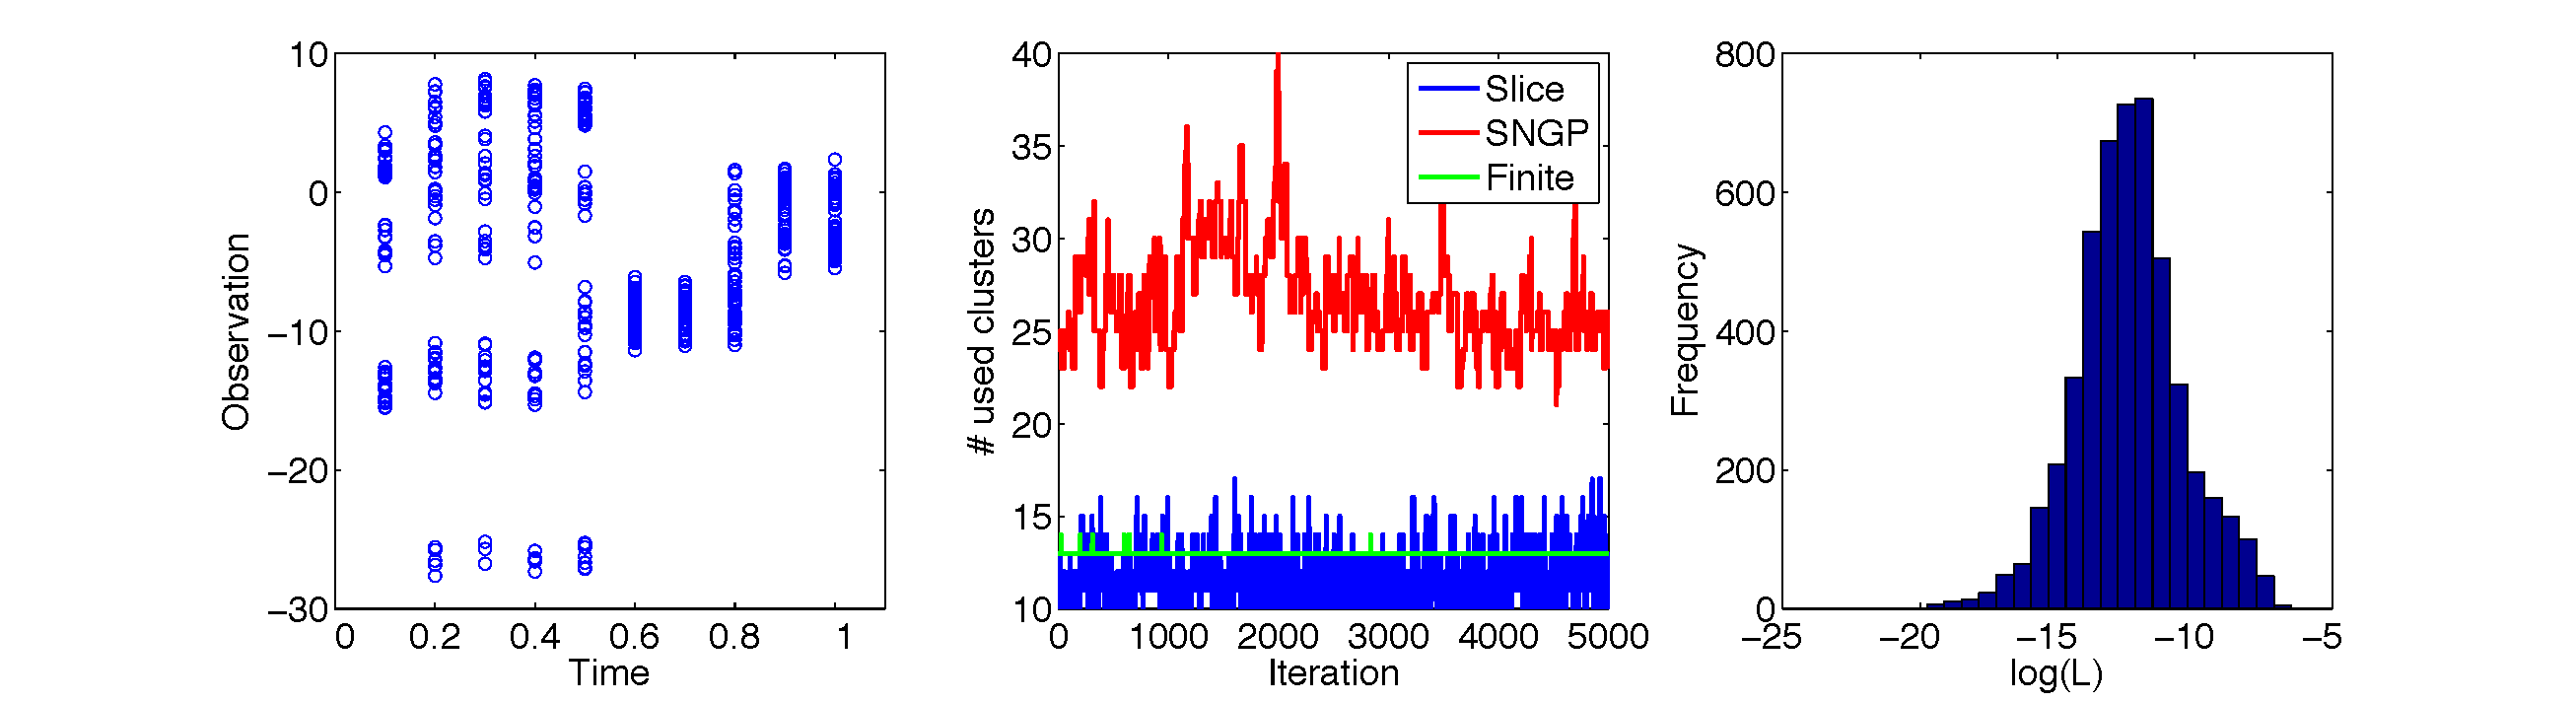
\includegraphics[scale=0.32]{figs/synth_stats.pdf}
  \end{center}
  \caption{Left: Synthetic data.  Middle: Trace plots of the number of clusters
  used by the three samplers.  Right: Histogram of truncation point $L$.
  }
  \label{fig:slicestats}
\end{figure}

We see that all three algorithms find a region of the posterior that gives
predictive estimates of a similar quality.  The autocorrelation estimates for 
the three samplers are also very similar. This might seem surprising, since the 
SNGP sampler uses sophisticated split-merge moves
to improve mixing, which have no analogue in the slice sampler. 
In addition, we note that although the per-iteration mixing performance is comparable, the average
time per $100$ iterations for the slice sampler was 
$\sim 10$ %$\sim 6$ 
seconds, for
the SNGP sampler was 
$\sim 30$ %$\sim 28$ 
seconds and for the finite sampler was 
$\sim 200$ %$\sim 194$ 
seconds. Even with only $100$ atoms the finite sampler
is much more expensive than the slice and SNGP\footnote{Sampling the cluster means
and assignments is the slowest step for the SNGP sampler taking about 3 seconds.
The times reported here only performed this step every 25 iterations
achieving reasonable results.  If this step were performed every iteration the
results may improve, but the computation time will explode.} samplers.

We also observe (Figure
\ref{fig:slicestats}) that both the slice and finite samplers
use essentially the true number of components underlying the data and that 
the SNGP sampler uses on average twice as many components.  The finite sampler finds a posterior mode with 13 clusters and rarely makes small moves from that
mode.  The slice sampler explores modes with 10-17 clusters, but never makes
large jumps away from this region.  The SNGP sampler explores the largest
number of used clusters ranging from 23-40, however, it has not explored
regions that use less clusters.

Figure \ref{fig:slicestats} also depicts the distribution
of the variable truncation level $L$ over all samples in the slice sampler. This suggests that a finite model that discards atoms with $\pi_k <
10^{-18}$ introduces negligible truncation error.  However, this value of $L$
corresponds to $\approx 10^{18}$ atoms in the finite model which is
computationally intractable.  To keep the computation times
reasonable we were only able to use $100$ atoms, a far cry
from the number implied by $L$.  

In Figure \ref{fig:preddens} (Left) we plot estimates of the predictive density
at each time stamp for the slice (a), finite (b) and SNGP (c) samplers.  All
three samplers capture the evolving structure of the distribution.  However,
the finite sampler seems unable to discard unneeded components.  This
is evidenced by the small mass of probability that spans times $[0,0.8]$ when
the data that the component explains only exists at times $[0.2,0.5]$.
The slice and SNGP samplers seem to both provide reasonable explanations for
the distribution, with the slice sampler tending to provide smoother estimates.

\subsection{Real data}
As well as providing an alternative inference method for existing models, our slice sampler can be used in a range of models that fall under the general class of KNRMs. To demonstrate this, we use the finite and slice versions of our sampler to learn two kernel DPs, one using a box kernel, $K(x,\mu) =
\idf{|x-\mu| < 0.2}$ (the setting in the SNGP), and the other using a square exponential kernel $K(x,\mu) = \exp(-200(x-\mu)^2)$, which has support
approximately on $[\mu-.2,\mu+.2]$.  The kernel was chosen to be somewhat
comparable to the box kernel, however, this kernel allows the influence of an
atom to diminish gradually as opposed to being constant. We compare to the SNGP sampler for the box kernel model, but note that this sampler is not applicable to the exponential kernel model.

We compare these approaches on two real-world datasets:
\begin{itemize}
  \item \textbf{Cosmic microwave background radiation (CMB)}\cite{Bennett:2003}: TT power spectrum measurements, $\eta$, from
the cosmic microwave background radiation (CMB) at various `multipole moments',
denoted $M$.  Both variables are
considered continuous and exhibit dependence.
We rescale $M$ to be in $[0,1]$ and standardize $\eta$ to have mean $0$ and
unit variance.
\item \textbf{Motorcycle crash data} \cite{Silverman:1985}.  This data set records the head acceleration, $A$, at various times
during a simulated motorcycle crash. We normalize time to $[0,1]$ and standardize $A$ to have
mean $0$ and unit variance.
\end{itemize}

Both datasets exhibit local heteroskedasticity, which cannot be captured using
the SNGP. For the CMB data, we consider only the first $600$ multipole moments, where the variance is approximately constant, allowing us to compare the SNGP sampler to the other algorithms. For all models we fixed the observation
variance to $0.02$, which we estimated from the standardized data.  To ease the 
computational burden of the samplers we picked $18$ time stamps in $[0.05,0.95]$,
equally spaced $0.05$ apart and assigned each observation to the time stamp
closest to its associated value of $M$.  This step is by no means necessary,
but the running time of the algorithms improves significantly. For the motorcycle data, there was no regime of constant variance, so we only compare the slice and finite
truncation samplers\footnote{The SNGP could still be used to model
this data, however, then we would be comparing the models as opposed to the
samplers.}.

For each dataset and each model/sampler, the held-out predictive log-likelihood, the mean number of used clusters and 
$\hat{\tau}$ are reported in  Table \ref{tab:mcmc}.  The
mixing characteristics of the chain are similar to those obtained for the
synthetic data.   We see in Table
\ref{tab:mcmc} that the box kernel and the square exponential kernel produce similar results on the CMB data. However, the kernel width was not optimized and different values may prove to yield superior results. For the motorcycle data we see a noticeable difference between using the box and square
exponential kernels where using the latter improves the held-out predictive
likelihood and results in both samplers using fewer components on average.

Figure \ref{fig:preddens} shows the predictive distributions obtained on the CMB data. Looking at the mean and $95\%$ CI of the predictive distribution (middle) we see that when using the box kernel the
SNGP actually fits the data the best.  This is most likely due to the fact that
the SNGP is using more atoms than the slice or finite samplers.  We show that the square exponential kernel (right) gives much smoother estimates and appears to fit the data
better, using the same number of atoms as were learned with the box kernel (see
Table \ref{tab:mcmc}).  We note that the slice sampler took 
$\sim 20$ %$\sim 14$
seconds per 100 iterations while the finite sampler used 
$\sim 150$ %$\sim 160$ 
seconds.  



%As with the CMB data we normalize time to $[0,1]$ and standardize $A$ to have
%mean $0$ and unit variance.  We use both the same box and square exponential
%kernels for this data as for the CMB dat.  We report the results in Table 
%\ref{tab:mcmc} where we see that for the box kernel the slice sampler has 
%found a region of the posterior with slightly better predictive likelihood.  In
%this case we see a noticeable difference between using the box and square
%exponential kernels where using the latter improves the held-out predictive
%likelihood and results in both samplers using fewer components on average.

\begin{figure}[t]
  \begin{center}
    \subfigure{
    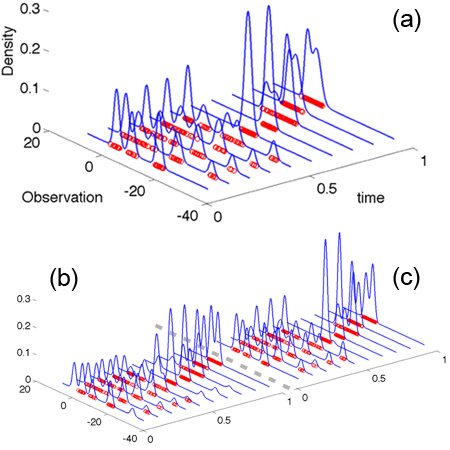
\includegraphics[bb=0 0 216 216,scale=0.5]{figs/synth_waterfall.pdf}
    }
    \subfigure{
    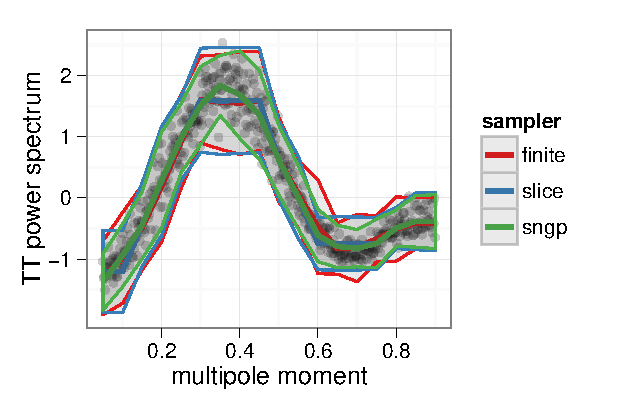
\includegraphics[bb=10 -15 300 184,scale=.48]{figs/cmb_box_predmean.pdf}
    }
    \subfigure{
    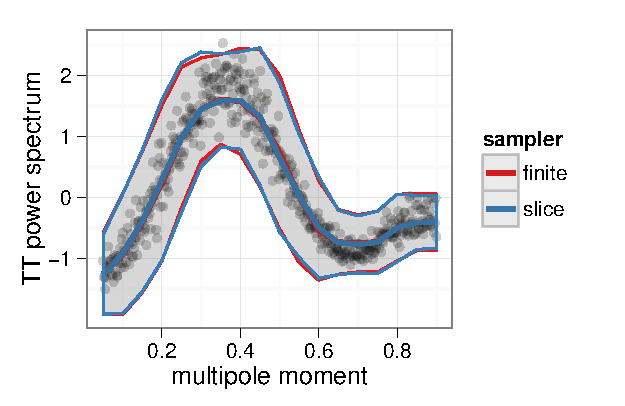
\includegraphics[bb=32 -15 300 184,scale=.48]{figs/cmb_se_predmean.pdf}
    }
  \end{center}
  \caption{\textbf{Left:} Predictive density at each time stamp for synthetic
  data using the slice (a), finite (b) and SNGP (c) samplers.  The scales of
  all three axis are identical.  \textbf{Middle:}
  Mean and $95\%$ CI of predictive distribution for all three
  samplers on CMB data using the box kernel.  \textbf{Right:} Mean and $95\%$
  CI of predictive distribution using the square exponential kernel.}
  \label{fig:preddens}
\end{figure}

\section{Conclusion}

%Something deep and impacting...

We presented the class of normalized kernel CRMs, a type of dependent 
normalized random measure.  This class generalizes previous work
by allowing more flexibility in the underlying CRM and kernel function used to
induce dependence.
We developed a slice sampler to perform inference on the infinite
dimensional measure and compared this method with samplers for a finite 
approximation and for the SNGP.  We found that the slice sampler yields
samples with competitive predictive accuracy at a fraction of the computational
cost.

There are many directions for future research.  
Incorporating
reversible-jump moves \cite{Green:Hastie:2009} such as split-merge proposals
should allow the slice sampler to explore larger regions of the parameter space
with a limited decrease in computational efficiency. A similar methodology may yield efficient inference algorithms for KCRMs such as the KBP, extending the existing slice sampler for the Indian Buffet Process
\cite{TehGorGha2007}.


\subsubsection*{Acknowledgments}
NF was funded by grant AFOSR FA9550-11-1-0166.  
SW was funded by grants NIH R01GM087694 and AFOSR FA9550010247.  

\newpage

\bibliography{nips2012}
\bibliographystyle{unsrt}

\end{document}